%!TEX root = ../main.tex
%%%%%%%%%%%%%%%%%%%%%%%%%%%%%%%%%%
% Links:
%
% Difficulty:
% Companies: 
%%%%%%%%%%%%%%%%%%%%%%%%%%%%%%%%%%


%\begin{figure}
%	\centering
%	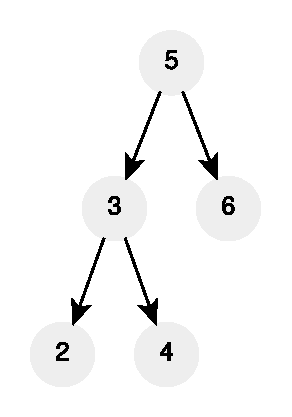
\includegraphics[width=\textwidth]{sources/binary_gap/images/example1}
%	\caption[Sample short cpation]{Sample Caption}.
%	\label{fig:binary_gap:example1}
%\end{figure}

\section{Binary gap}
\label{ch:binary_gap}

\section{Problem statement}
\begin{exercise}
\label{example:binary_gap:exercice1}
A binary gap within a positive integer $n$ is any maximal sequence of consecutive zeros that is surrounded by ones at both ends in the binary representation of n.

For example, number 9 has binary representation 1001 and contains a binary gap of length 2. The number 529 has binary representation 1000010001 and contains two binary gaps: one of length 4 and one of length 3. The number 20 has binary representation 10100 and contains one binary gap of length 1. The number 15 has binary representation 1111 and has no binary gaps. The number 32 has binary representation 100000 and has no binary gaps.

Write a function:

int solution(int n);

that, given a positive integer n, returns the length of its longest binary gap. The function should return 0 if n doesn't contain a binary gap.

For example, given n = 1041 the function should return 5, because n has binary representation 10000010001 and so its longest binary gap is of length 5. Given n = 32 the function should return 0, because n has binary representation '100000' and thus no binary gaps.

Write an efficient algorithm for the following assumptions:

n is an integer within the range 1..MAXINT.
	%example1
	\begin{example}
		\label{example:binary_gap:example1}
		\hfill \\
	
		
	\end{example}

	%example2
	\begin{example}
		\label{example:binary_gap:example2}
		\hfill \\
		
	\end{example}

\end{exercise}

\section{Clarification Questions}

\begin{QandA}
	\item 
	\begin{answered}
		\textit{}
	\end{answered}
	
\end{QandA}

\section{Discussion}
\label{binary_gap:sec:discussion}


\subsection{Brute-force}
\label{binary_gap:sec:bruteforce}

\lstinputlisting[language=c++, caption={Sample Caption},label=list:binary_gap]{sources/binary_gap/binary_gap_solution1.cpp}

\lstinputlisting[language=c++, caption={Sample Caption},label=list:binary_gap]{sources/binary_gap/binary_gap_solution2.cpp}

